%*----------- SLIDE -------------------------------------------------------------
\begin{frame}[t]{Lei de Moore}
        \begin{columns}
            \column{.5\textwidth}
                \begin{figure}
                    \roundpic[xshift=1cm,yshift=0cm]{5.8cm}{9cm}{moore.jpeg}
                 %\caption{.}
                \end{figure}
            \column{.48\textwidth}
            \LARGE
            "A densidade de transistores em um chip dobra a cada 18 meses mantendo o mesmo custo de fabricação."\\
            Gordon E. Moore, 1965
            \column{.02\textwidth}
        \end{columns}
        %\column{.01\textwidth}
%*----------- notes
    \note[item]{Notes can help you to remember important information. Turn on the notes option.}
\end{frame}
% %*----------- SLIDE -------------------------------------------------------------
\begin{frame}[t]{Lei de Moore}
    \begin{columns}
        \column{.6\textwidth}
        \begin{figure}
            \centering
            \textbf{Evolução dos Microprocessadores}\par\medskip
            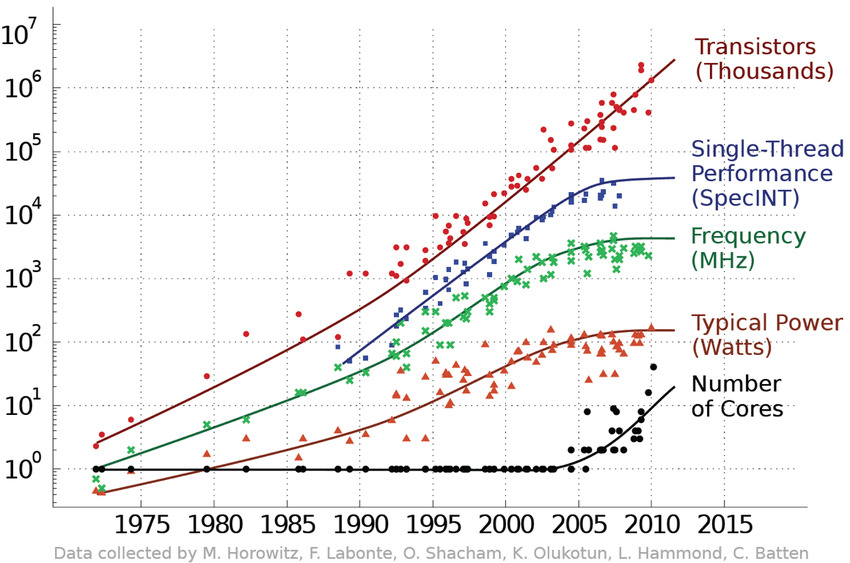
\includegraphics[trim = 0 20 0 0, clip, width=1
            \textwidth]{trends.jpg}
            %\caption{.}
        \end{figure}
        \column{.4\textwidth}
        \large{
        \begin{itemize}
            \item O número de transistores por chip cresceu em progressão geométrica\\
            \item O aumento no número de transistores parou de refletir no aumento da performance\\
            \item O consumo energético se tornou muito alto
        \end{itemize}
        }
    \end{columns}
    
        %\column{.01\textwidth}
%*----------- notes
    \note[item]{Notes can help you to remember important information. Turn on the notes option.}
\end{frame}
% %*----------- SLIDE -------------------------------------------------------------
\begin{frame}
    \begin{center}
        \vspace*{1.5cm}
        \justifying
        \huge{“Se um único computador (processador) consegue resolver um problema N segundos, podem N computadores (processadores) resolver o mesmo problema em 1 segundo?”}
    \end{center}
\end{frame}
% %*----------- SLIDE -------------------------------------------------------------
\begin{frame}[t]{Programação em paralelo}
    \framesubtitle{Porquê usar GPUs?}
    \begin{columns}
        \column{.6\textwidth}
        \begin{figure}
            \centering
            \textbf{Performance das GPUs vs CPUs em GFLOPS/s}\par\medskip
            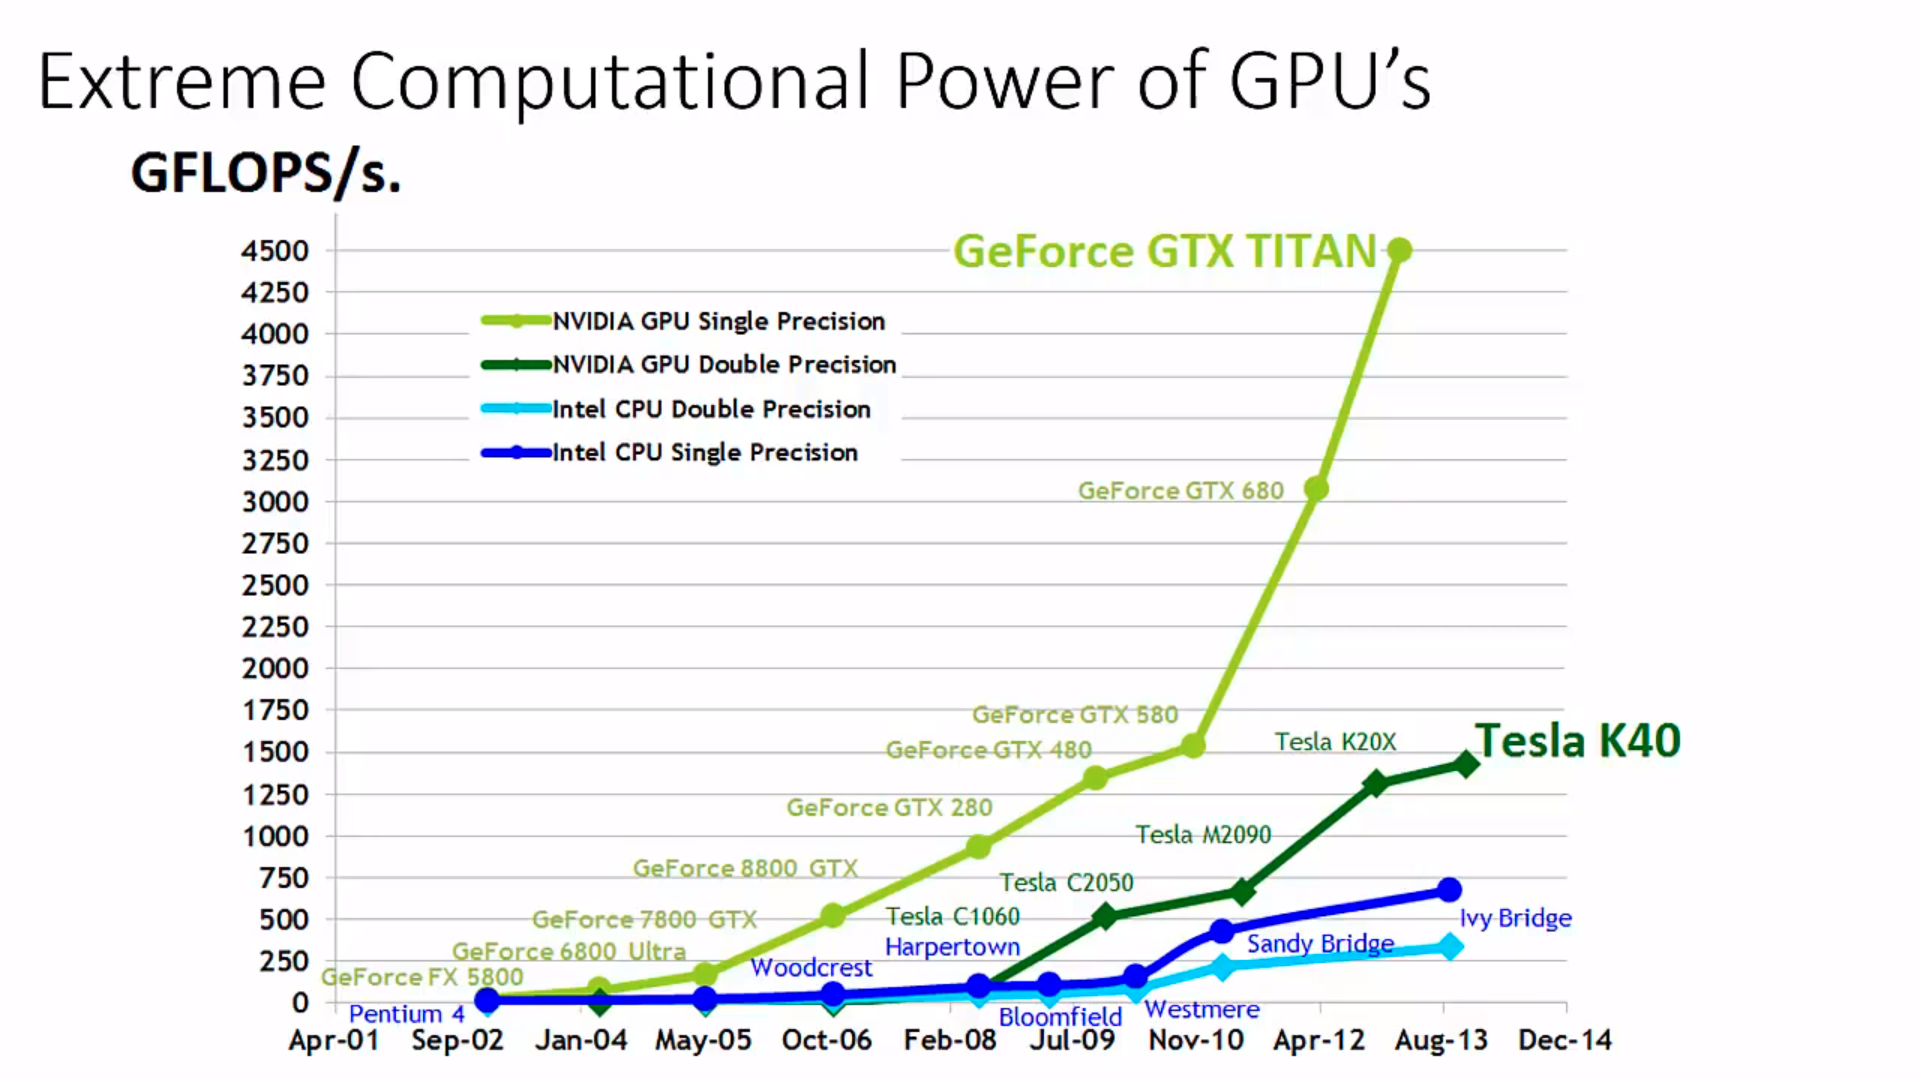
\includegraphics[trim = 200 10 210 210, clip, width=1
            \textwidth]{gpuvccpu.png}
        \end{figure}
        \column{.4\textwidth}
        \vspace*{0.4cm}
        \itemize
        \item Poder computacional muito superior das GPUs
        \item A performance das GPUs cresce muito mais rápido do que a das CPUs
        \item Reduzir o tempo de solução de um problema
        \item Resolver problemas mais complexos
    \end{columns}
        
        %\column{.01\textwidth}
%*----------- notes
    \note[item]{Notes can help you to remember important information. Turn on the notes option.}
\end{frame}
%*----------- SLIDE -------------------------------------------------------------
\begin{frame}[t]{CPU x GPU}
    \framesubtitle{Qual a diferença?}
    \begin{figure}
        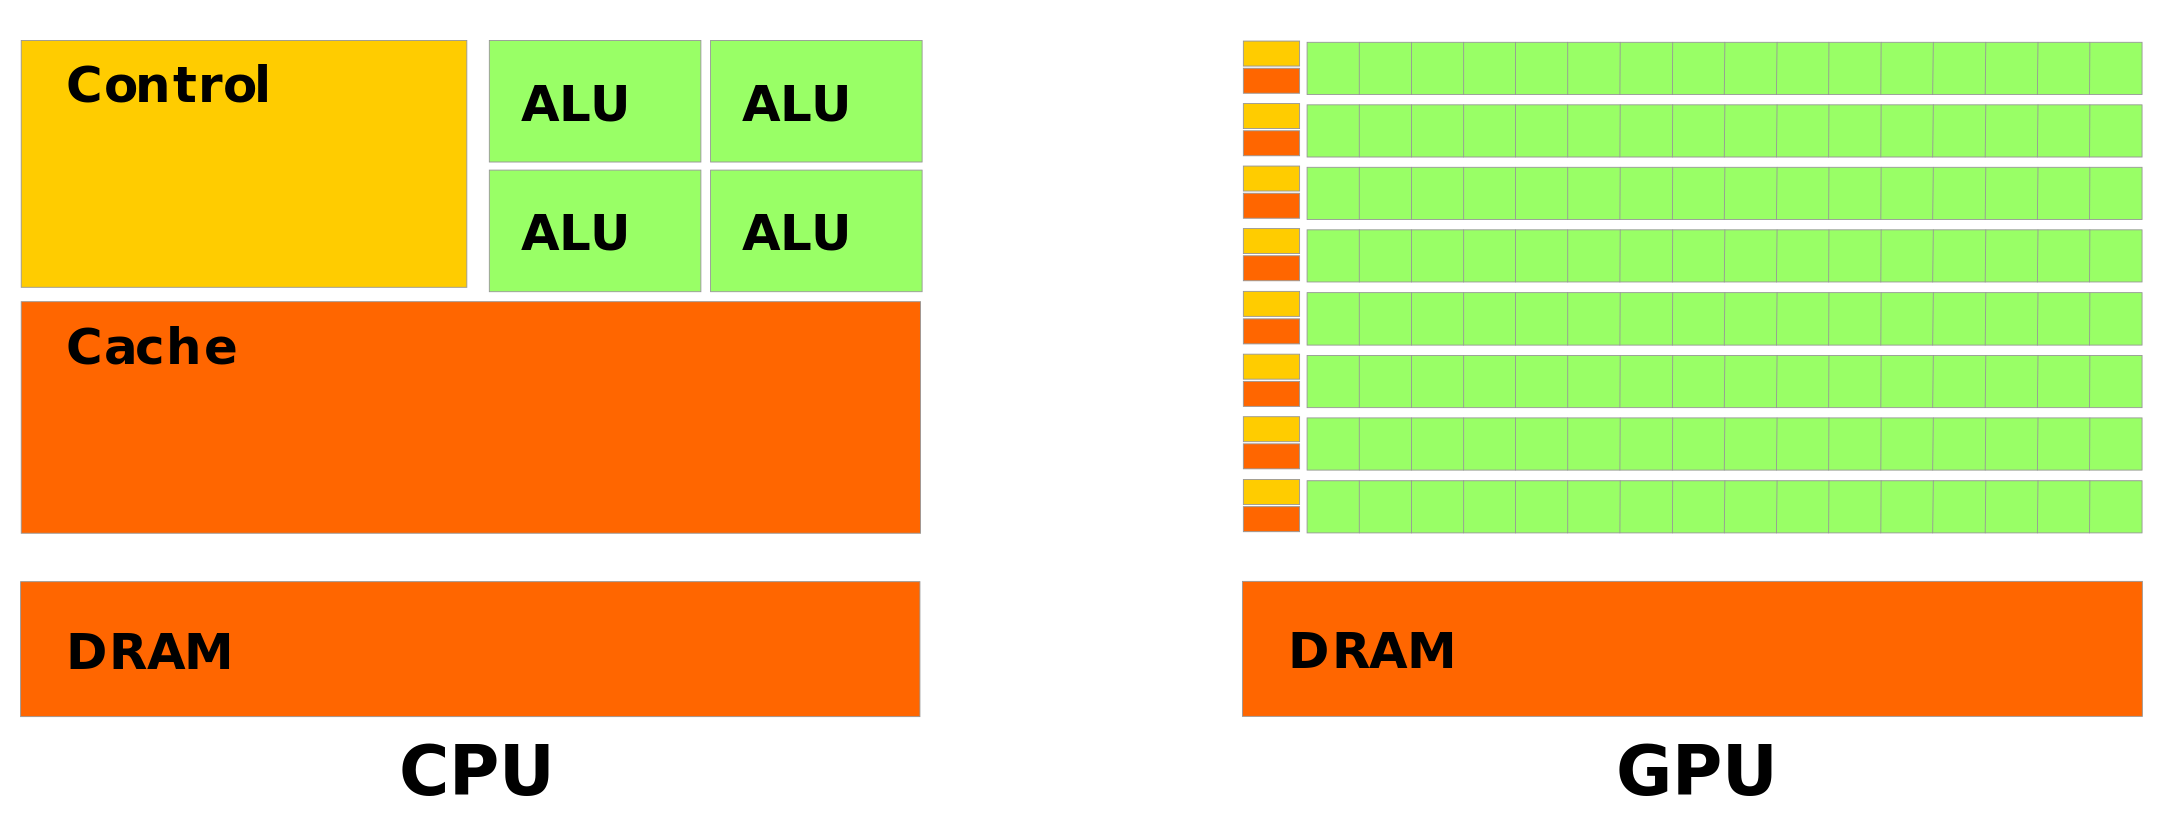
\includegraphics[trim = 0 0 0 0, clip, width=1\textwidth]{Cpu-gpu.png}
        %\caption{.}
    \end{figure}

%*----------- notes
    \note[item]{Notes can help you to remember important information. Turn on the notes option.}
\end{frame}
% %*----------- SLIDE -------------------------------------------------------------
\begin{frame}[t]{O que é CUDA?}
    \framesubtitle{Compute Unified Device Architecture}
    \begin{columns}
        \column{.02\textwidth}
        \column{.48\textwidth}
            % \vspace{.4cm}
            \Large
            \begin{itemize}
                \item É um modelo de programação em paralelo que permite o uso das GPUs da Nvidia
                \item É basicamente C/C++ com algumas extensões
                \item Pode ser usado em outras linguagens como Fortran e Python 
            \end{itemize}
        \column{.48\textwidth}
            \begin{figure}
                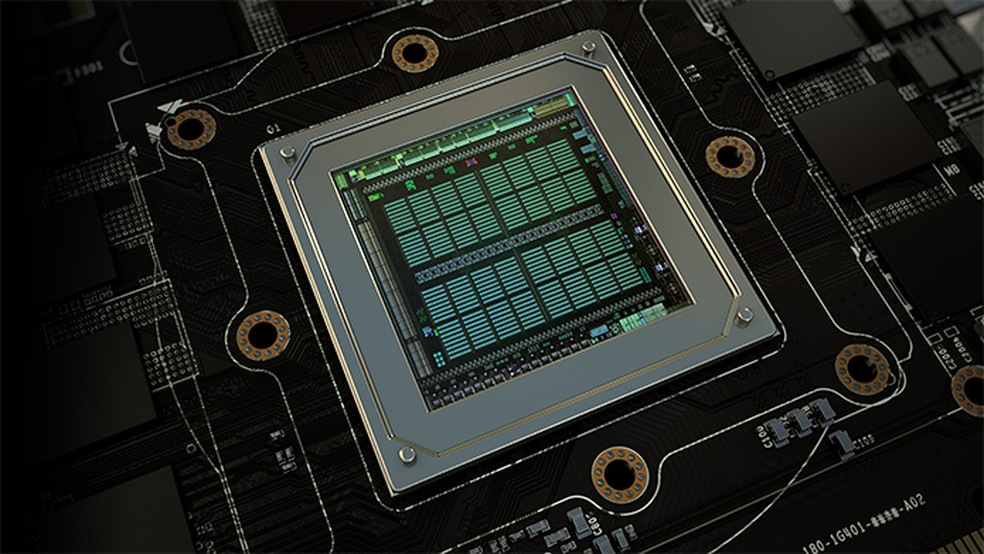
\includegraphics[trim = 180 0 150 0, clip, width=.9
                \textwidth]{2017-04-12-nvidia-gpu.jpeg}
                %\caption{.}
            \end{figure}  
        \column{.02\textwidth}      
    \end{columns}
        %\column{.01\textwidth}
%*----------- notes
    \note[item]{Notes can help you to remember important information. Turn on the notes option.}
\end{frame}
% %*----------- SLIDE -------------------------------------------------------------
\begin{frame}[t]{Aplicações}
    \begin{columns}
        \column{.02\textwidth}
        \column{.48\textwidth}
            % \vspace{.4cm}
            \Large
            \begin{itemize}
                \item Processamento de imagens
                \item Simulações
                \item Cálculos vetoriais e matriciais
                \item Algoritimos de buscas
                \item Química computacional
                \item Ordenação
                \item Inteligência computacional
                \item Deep learning
            \end{itemize}
        \column{.48\textwidth}
            \begin{figure}
                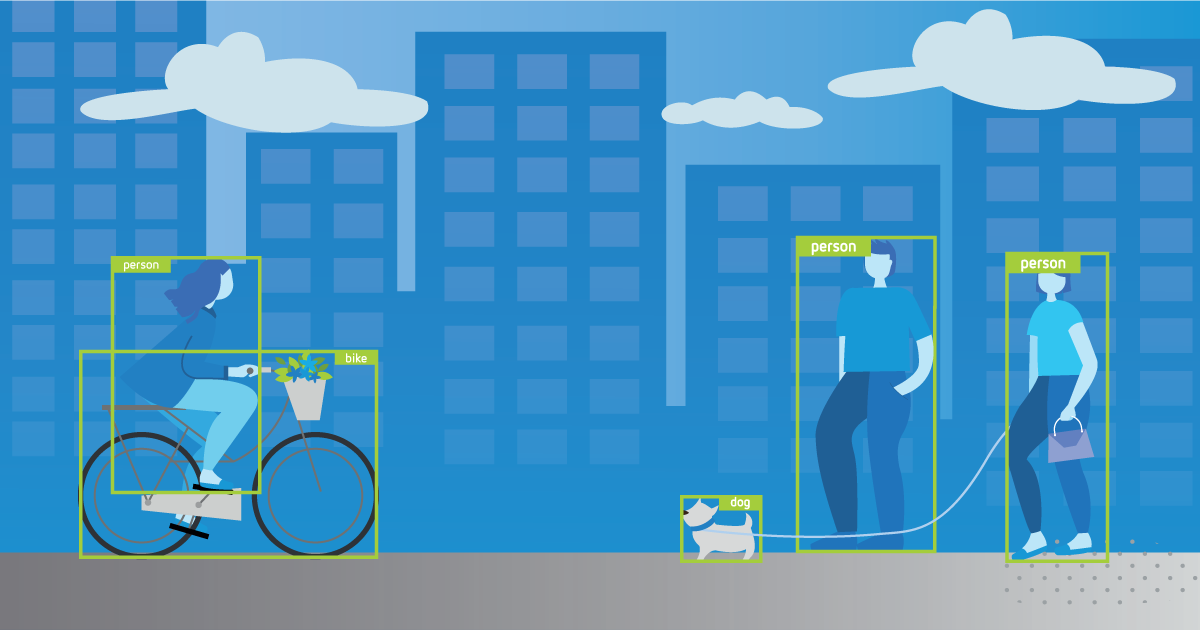
\includegraphics[trim = 600 0 0 0, clip, width=.85
                \textwidth]{object-detection-illustration.png}
                %\caption{.}
            \end{figure}  
        \column{.02\textwidth}      
    \end{columns}
        %\column{.01\textwidth}
%*----------- notes
    \note[item]{Notes can help you to remember important information. Turn on the notes option.}
\end{frame}
%*----------- SLIDE -------------------------------------------------------------
\begin{frame}[t]{Nvidia G80}
    \framesubtitle{GeForce 8800}
    \begin{figure}
        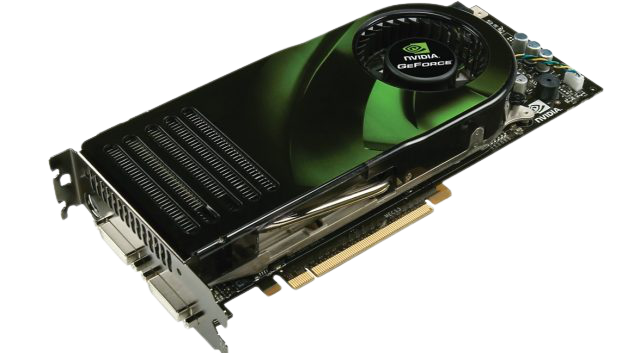
\includegraphics[trim = 0 0 0 0, clip, width=1\textwidth]{g80.png}
        %\caption{.}
    \end{figure}

%*----------- notes
    \note[item]{Notes can help you to remember important information. Turn on the notes option.}
\end{frame}
%*----------- SLIDE -------------------------------------------------------------
\begin{frame}[t]{Conceitos Iniciais}
    % \framesubtitle{Lei de Zipf}
    \LARGE{
    \textbf{Kernel}\\
    }
    \large{
    $\hookrightarrow$ É o código que é executado na GPU\\
    }
    \LARGE{
    \textbf{Thread}\\
    }
    \large{
    $\hookrightarrow$ É a execução do Kernel em um único pedaço dos dados que é executada em um CUDA Core\\
    }
    \LARGE{
    \textbf{Thread Block}\\
    }
    \large{
    $\hookrightarrow$ É um conjunto de Threads executado em uma Streaming Multiprocessor (SM)\\
    }
    \LARGE{
    \textbf{Grid}\\
    }
    \large{
    $\hookrightarrow$É um conjunto de Blocks que é executada em toda GPU apartir do launch do Kernel
    }
    % \large{
    % \itemize
    % \item É um conjunto de Blocks que é executada em toda GPU apartir do launch do Kernel\\
    % }
%*----------- notes
    \note[item]{Notes can help you to remember important information. Turn on the notes option.}
\end{frame}
%*----------- SLIDE -------------------------------------------------------------
\begin{frame}[t]{Arquitetura CUDA}
    % \framesubtitle{Lei de Zipf}
    \begin{columns}
        \column{.15\textwidth}
        \column{.35\textwidth}
            \begin{figure}
               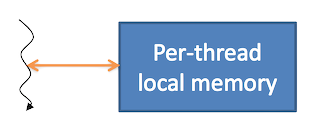
\includegraphics[trim = 0 0 0 0, clip, width=1\textwidth]{02-localmemory-removebg-preview.png}
            \end{figure}
        \column{.35\textwidth}
            \begin{figure}
               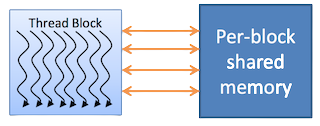
\includegraphics[trim = 0 0 0 0, clip, width=1\textwidth]{02-sharedmemory-removebg-preview.png}
            \end{figure}
        \column{.15\textwidth}    
    \end{columns}
    \begin{figure}
        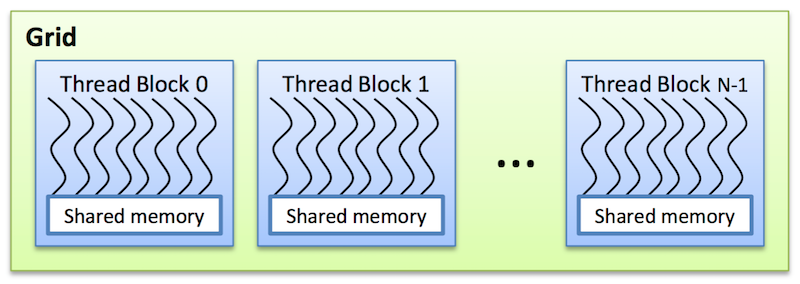
\includegraphics[trim = 0 0 0 0, clip, width=0.7\textwidth]{02-threadgrid.png}
    \end{figure}
%*----------- notes
    \note[item]{Notes can help you to remember important information. Turn on the notes option.}
\end{frame}
% %*----------- SLIDE -------------------------------------------------------------
\begin{frame}[t]{Arquitetura CUDA}
    % \framesubtitle{Qual a diferença?}
    \begin{figure}
        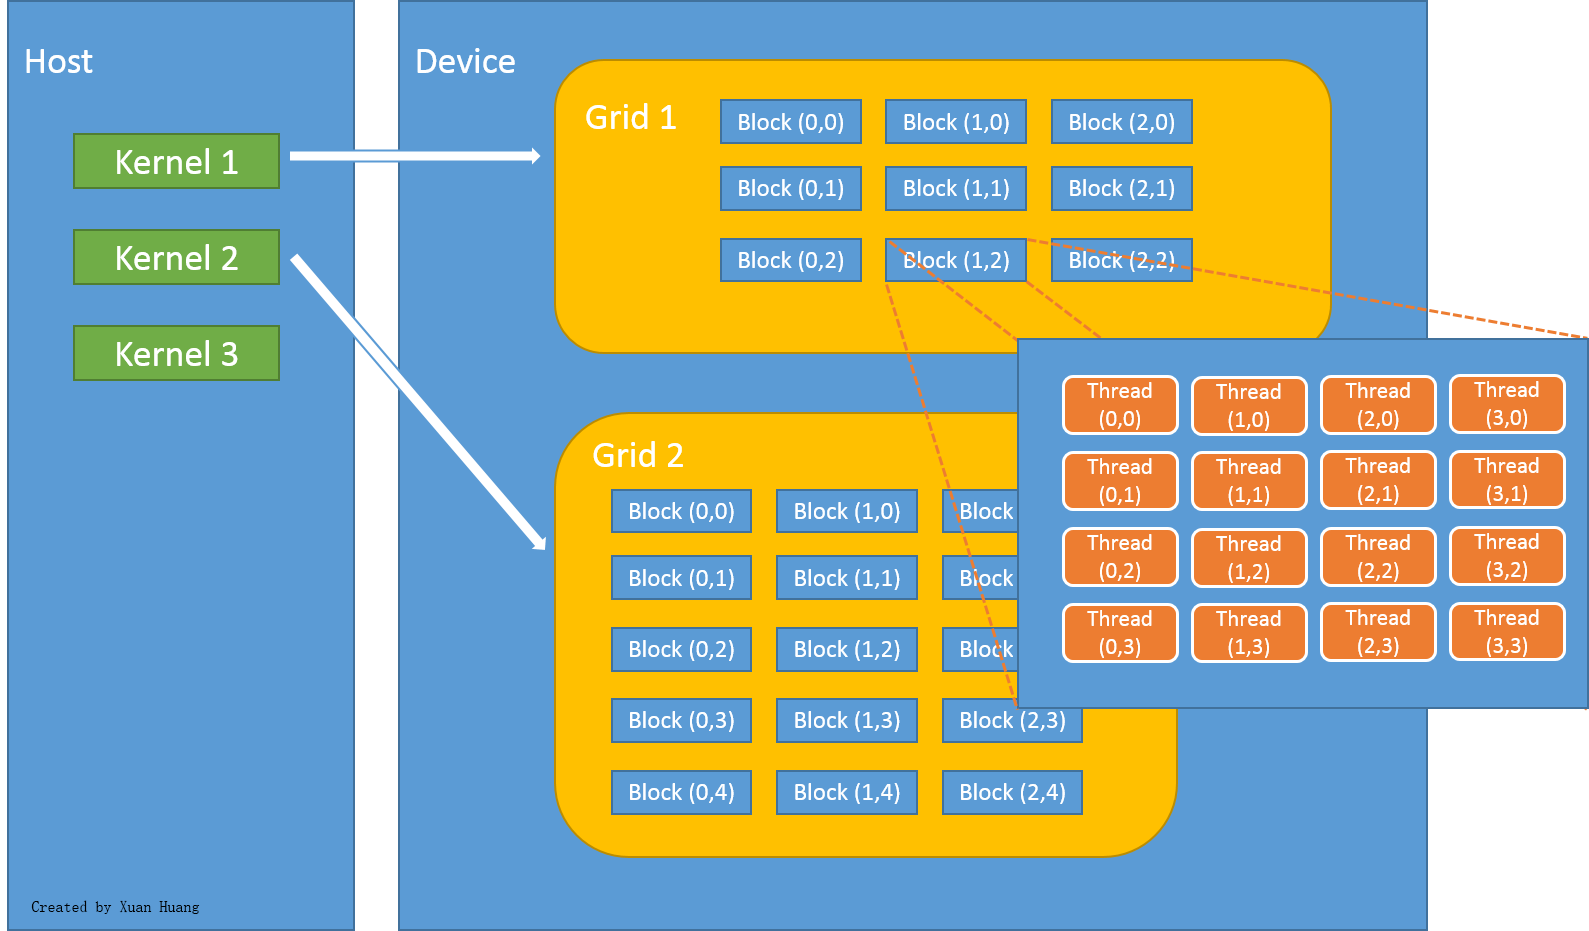
\includegraphics[trim = 0 0 0 0, clip, width=0.78\textwidth]{threadblock.png}
        %\caption{.}
    \end{figure}

%*----------- notes
    \note[item]{Notes can help you to remember important information. Turn on the notes option.}
\end{frame}
% %*----------- SLIDE -------------------------------------------------------------
\begin{frame}[t]{Programação Heterogênea}
    \framesubtitle{Host + Device}
    \begin{figure}
        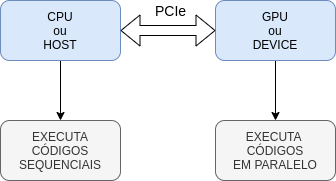
\includegraphics[trim = 0 0 0 0, clip, width=0.7\textwidth]{het.png}
        %\caption{.}
    \end{figure}

%*----------- notes
    \note[item]{Notes can help you to remember important information. Turn on the notes option.}
\end{frame}
% %*----------- SLIDE -------------------------------------------------------------
\begin{frame}[t]{Block Index e Thread Index}
    % \framesubtitle{Qual a diferença?}
    \textbf{\Large{ThreadIdx}} $\rightarrow$ Index da Thread\\
    Cada thread tem um ID único no Block. Em um Block 3D, tem 3 componentes:\\
    ThreadIdx.x\\
    ThreadIdx.y\\
    ThreadIdx.z\\
    \vspace*{0.5cm}
    \textbf{\Large{BlockIdx}} $\rightarrow$ Index do Block\\
    Cada Block tem um ID único no Grid. Em um Grid 3D, tem 3 componentes:\\
    BlockIdx.x\\
    BlockIdx.y\\
    BlockIdx.z\\

%*----------- notes
    \note[item]{Notes can help you to remember important information. Turn on the notes option.}
\end{frame}
% %*----------- SLIDE -------------------------------------------------------------
\begin{frame}[t]{Modelo de Memória}
    % \framesubtitle{Qual a diferença?}
    \begin{columns}
        \column{0.5\textwidth}
            \begin{figure}
                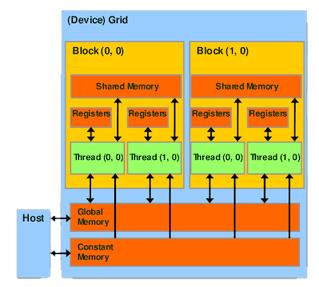
\includegraphics [trim = 0 0 0 0, clip, width=1\textwidth]{MEMORYY.png}
                %\caption{.}
            \end{figure}    
        \column{0.5\textwidth}
        \itemize
        \item O host se comunica com o device através da memória global
        \item Apenas threads de um mesmo Block podem se comunicar e cooperar através da memória compartilhada
        \item Therds de blocks diferentes não se comunicam
        \item Cada thread possui um conjunto de registradores e uma memória local
    \end{columns}
    % \begin{figure}
    %     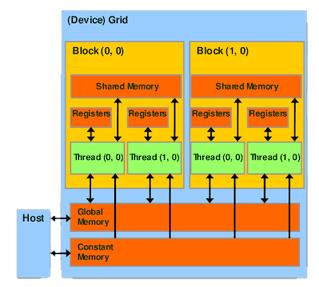
\includegraphics [trim = 0 0 0 0, clip, width=0.5\textwidth]{MEMORYY.png}
    %     %\caption{.}
    % \end{figure}

%*----------- notes
    \note[item]{Notes can help you to remember important information. Turn on the notes option.}
\end{frame}
% %*----------- SLIDE -------------------------------------------------------------
\begin{frame}[t]{Modelo de Memória}
    \framesubtitle{Cooperação em Thread Blocks}
    \begin{columns}
        \column{.05\textwidth}
        \column{.45\textwidth}
            \begin{figure}
               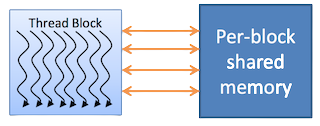
\includegraphics[trim = 0 0 0 0, clip, width=0.9\textwidth]{02-sharedmemory-removebg-preview.png}
            \end{figure}
        
        \column{.5\textwidth}
            \begin{figure}
               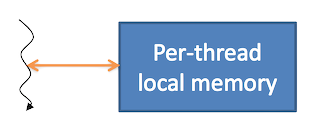
\includegraphics[trim = 0 0 0 0, clip, width=0.9\textwidth]{02-localmemory-removebg-preview.png}
            \end{figure}
        \column{.15\textwidth}    
    \end{columns}
    \vspace*{0.2cm}
    \itemize
    \item Threads podem compartilhar resultados entre si ou cooperar para produzir um resultado único através da memória compartilhada
    \item Threads podem se sincronizar umas com as outras
    \item A memória local é privada para cada thread
    \item A memória compartilhada é mais rápida que a memória global e a local
    % \begin{figure}
    %     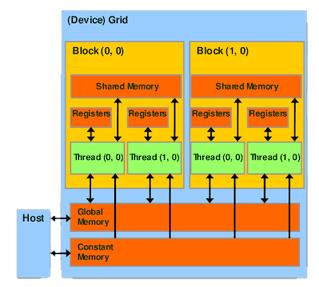
\includegraphics [trim = 0 0 0 0, clip, width=0.5\textwidth]{MEMORYY.png}
    %     %\caption{.}
    % \end{figure}

%*----------- notes
    \note[item]{Notes can help you to remember important information. Turn on the notes option.}
\end{frame}
% %*----------- SLIDE -------------------------------------------------------------
\begin{frame}[t]{Modelo de memória}
    % \framesubtitle{Qual a diferença?}
    \begin{figure}
        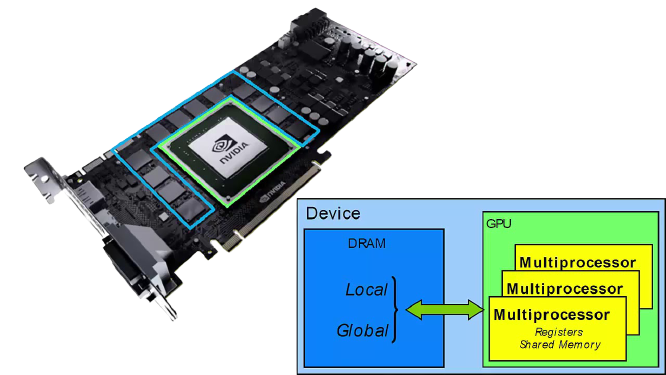
\includegraphics[trim = 0 0 0 0, clip, width=0.78\textwidth]{maxresdefault-removebg-preview.png}
        %\caption{.}
    \end{figure}

%*----------- notes
    \note[item]{Notes can help you to remember important information. Turn on the notes option.}
\end{frame}
% %*----------- SLIDE -------------------------------------------------------------
\begin{frame}[t]{Kernel Mínimo}
    % \framesubtitle{Cooperação em Thread Blocks} 
    \Large{
    \begin{shaded}

        \textunderscore \textunderscore  global\textunderscore \textunderscore void mykernel(...)\{\\
        \}
        % \{\\
        % \;\;\;\; int idx = blockDim.x * blockIdx.x + threadIdx.x\\
        % \;\;\;\; a[idx] = 13\\
        % \} \\
    \end{shaded}
    }
    \Large{
    \justifying{
    A keyword \textcolor{red}{\textunderscore \textunderscore  global\textunderscore \textunderscore} indica uma função que é executada no device.\\ %e é chamada pelo host.\\
    O compilador nvcc separa o código em componentes de host e componentes de device. Os componentes de device são compilados com o nvcc e os componentes de host por compiladores padrão como gcc.
    }
    }
    
    % \begin{figure}
    %     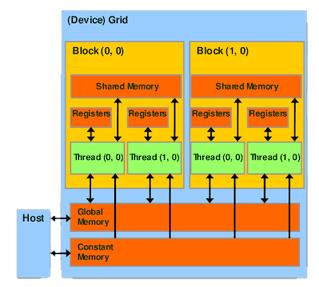
\includegraphics [trim = 0 0 0 0, clip, width=0.5\textwidth]{MEMORYY.png}
    %     %\caption{.}
    % \end{figure}
%*----------- notes
    \note[item]{Notes can help you to remember important information. Turn on the notes option.}
\end{frame}
% %*----------- SLIDE -------------------------------------------------------------
\begin{frame}[t]{Alocação de Memória}
    % \framesubtitle{Cooperação em Thread Blocks} 
    \Large{
    \begin{shaded}
        \itemize
        \item cudaMalloc() $\rightarrow$ Aloca espaço para cópias no Device\\
        \item cudaMemcpy() $\rightarrow$ Copia entradas do Host pro Device ou do Device pro Host\\
        \item cudaFree() $\rightarrow$ Desaloca memória no Device\\
        % \item cudaMenset() $\rightarrow$ ?
    % \end{shaded}
    %     $\rightarrow$ Copia entradas para o device\\
    % \begin{shaded}
        % \itemize
        % \item cudaMalloc(void *pointer, size\textunderscore t nbytes)\\
        % \item cudaMenset(void *pointer, int value, size\textunderscore t count)\\
        % \item cudaFree(void* pointer)
        % \item cudaMemcpy()
    \end{shaded}
    }
    
    % \begin{figure}
    %     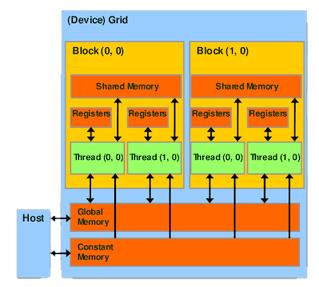
\includegraphics [trim = 0 0 0 0, clip, width=0.5\textwidth]{MEMORYY.png}
    %     %\caption{.}
    % \end{figure}
%*----------- notes
    \note[item]{Notes can help you to remember important information. Turn on the notes option.}
\end{frame}
% %*----------- SLIDE -------------------------------------------------------------
\begin{frame}[t]{Alocação de Memória}
    \framesubtitle{cudaMalloc e cudaFree} 
    \Large{
    \begin{shaded}
        cudaMalloc(LOCATION, SIZE);\\
        cudaMalloc((void **)\&d\textunderscore a, sizeof(int));
    \end{shaded}
    }
    \begin{itemize}
        \item O primeiro argumento é a localização da memória no device para alocar dados
        \item O segundo argumento é o tamanho dos dados em bytes
    \end{itemize}
    \begin{shaded}
        cudaFree(d\textunderscore a);$\rightarrow$ Desaloca memória
    \end{shaded}
    % \begin{figure}
    %     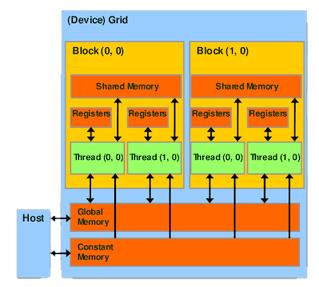
\includegraphics [trim = 0 0 0 0, clip, width=0.5\textwidth]{MEMORYY.png}
    %     %\caption{.}
    % \end{figure}
%*----------- notes
    \note[item]{Notes can help you to remember important information. Turn on the notes option.}
\end{frame}
% %*----------- SLIDE -------------------------------------------------------------
\begin{frame}[t]{Alocação de Memória}
    \framesubtitle{cudaMemcpy} 
    \Large{
    \begin{shaded}
        cudaMemcpy(dst,src,size,direction);\\ %source destination
        cudaMemcpy(d\textunderscore a, a, size,cudaMemcpyHostToDevice);
    \end{shaded}
    }
    \large{
    \begin{itemize}
        \item O primeiro e o segundos argumento são os pointers do endereço que vai receber a cópia e do que vai enviar a cópia, respectivamente
        \item O terceiro argumento é o tamanho em bytes
        \item O quarto elemento é a direção, podendo ser:\\$\hookrightarrow$ \textcolor{red}{cudaMemcpyHostToDevice}\\$\hookrightarrow$ \textcolor{red}{cudaMemcpyDeviceToHost}
    \end{itemize}
    }

    % \begin{figure}
    %     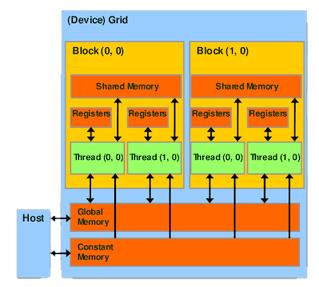
\includegraphics [trim = 0 0 0 0, clip, width=0.5\textwidth]{MEMORYY.png}
    %     %\caption{.}
    % \end{figure}
%*----------- notes
    \note[item]{Notes can help you to remember important information. Turn on the notes option.}
\end{frame}
% %*----------- SLIDE -------------------------------------------------------------
\begin{frame}[t]{Launching do Kernel}
    % \framesubtitle{Cooperação em Thread Blocks}
    \Large{
    \begin{shaded}
        dim3 grid\textunderscore size(x,y,z);\\
        dim3 block\textunderscore size(x,y,z);\\
        kernel\textless \textless \textless grid\textunderscore size, block\textunderscore size\textgreater \textgreater \textgreater (...);
    \end{shaded}
    }
    \justifying
    O primeiro parâmetro e o segundo parâmetro se referem ao tamanho e a configuração do Grid e dos Blocks. Ambos parâmetros podem ser 1D, 2D ou 3D.
%*----------- notes
    \note[item]{Notes can help you to remember important information. Turn on the notes option.}
\end{frame}
% %*----------- SLIDE -------------------------------------------------------------
\begin{frame}[t]{Instalando CUDA no Ubuntu 20.04}
    % \framesubtitle{Cooperação em Thread Blocks}
    \Large{
    \begin{shaded}
        \$ sudo apt update\\
        \$ sudo apt install build-essential\\ 
        \$ sudo apt install nvidia-cuda-toolkit\\
    \end{shaded}
    }
    \justifying
    O segundo comando instala o compilador GCC, GNU Compiler Collection, o compilador de códigos em C/C++ e o terceiro comando instala o compilador NVCC, Nvidia CUDA Compiler.
%*----------- notes
    \note[item]{Notes can help you to remember important information. Turn on the notes option.}
\end{frame}
% %*----------- SLIDE -------------------------------------------------------------
\begin{frame}[t]{Compilando Códigos e Executando}
    % \framesubtitle{Cooperação em Thread Blocks}
    \Large{
    \begin{shaded}
        \$ nvcc -o hello hello.cu \\
        \$ ./hello 
    \end{shaded}
    }
    \justifying
    O primeiro comando compila o código hello.cu e o segundo o executa o código binário compilado hello.
%*----------- notes
    \note[item]{Notes can help you to remember important information. Turn on the notes option.}
\end{frame}